\chapter{Estado del arte}
\section{Introducción}
En este capítulo, se abordará el estado del arte en
cuanto a aplicaciones móviles para la colaboración y
actividades en grupo, destacando las características y
funcionalidades más relevantes de las soluciones existentes.
Se analizarán las oportunidades de mejora en las aplicaciones actuales y cómo nuestra propuesta pretende llenar esos vacíos, 
enfatizando la importancia de comprender el mercado objetivo para lanzar una aplicación que no solo sea útil y atractiva, 
sino que también logre destacarse y consolidarse en el mercado.

\section{Estado del arte}

Antes de pasar a explicar las soluciones existentes es importante describir el problema que se está tratando de resolver.

Los jóvenes de hoy en día pasan un tiempo significativo de su día a día interactuando con sus dispositivos móviles. 
Según la organización sin ánimo de lucro Common Sense Media, los adolescentes de 13 a 18 años 
pasan un promedio de 8 horas y 39 minutos al día en sus dispositivos, 
mientras que los niños de 8 a 12 años pasan un promedio de 5 horas y 33 minutos al día en sus dispositivos\cite{REF13}.
Un 17\verb|%| de crecimiento en el tiempo de pantalla de los adolescentes en comparación con 2019.
\begin{figure}[H]
  \centering
  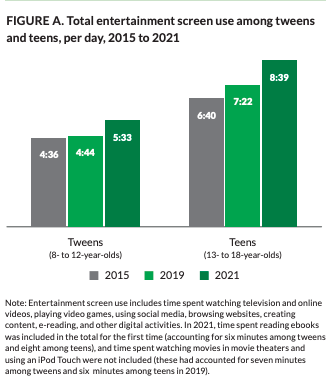
\includegraphics[width=0.7\linewidth]{images/estadodelarte/screentimeteens.png}
  \caption{Tiempo de pantalla de los adolescentes}
  \label{fig:tiempo_pantalla}
\end{figure}
Por consiguiente, surge una interrogante fundamental respecto al impacto adverso que el excesivo tiempo frente a la pantalla puede ejercer sobre la esfera social de los jóvenes. 
Se plantea la hipótesis de que la inversión de tiempo en dispositivos digitales, en detrimento de la participación en actividades sociales tangibles, 
podría comprometer el desarrollo de competencias esenciales tales como liderazgo, colaboración y habilidades interpersonales. 
Se observa una tendencia a social sobre importancia de priorizar la interacción humana directa, reconociendo su valor intrínseco y su papel en el fortalecimiento del tejido social.

\begin{figure}[H]
  \centering
  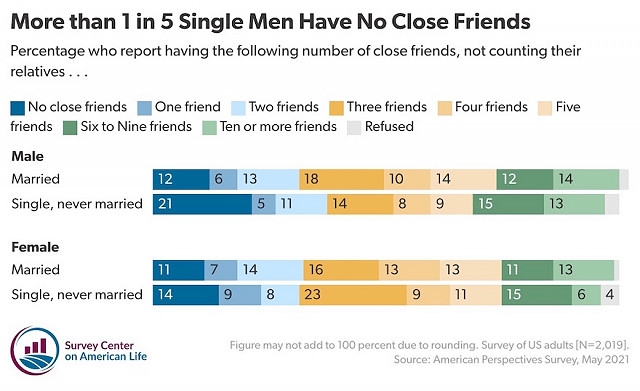
\includegraphics[width=0.7\linewidth]{images/estadodelarte/noclosefriends.jpeg}
  \caption{Más de 1 de cada 5 hombres solteros no tienen amigos cercanos}
  \label{fig:no_close_friends}
\end{figure}

También otra estadística llamativa es que más de 1 de cada 5 hombres solteros no tienen amigos cercanos, 
por lo menos en Estados Unidos, según un estudio el Survey Center on American Life\cite{REF14}.

Aunque es difícil medir el aislamiento social y la soledad de manera precisa, existe una fuerte evidencia de que muchos adultos de 50 años de edad o más están socialmente aislados 
o se sienten solos en maneras que ponen en riesgo su salud. 
Estudios recientes han revelado que el aislamiento social aumenta significativamente el riesgo de morir prematuramente por todas las causas, 
un riesgo que podría rivalizar con el del tabaquismo, la obesidad y la inactividad física. Además, el aislamiento social se ha asociado a un aumento de casi el 50\% del 
riesgo de demencia, mientras que las relaciones sociales escasas se han vinculado a un aumento del 29\% del riesgo de enfermedad cardiaca y a un 
aumento del 32\% del riesgo de accidente cerebrovascular. La soledad también se ha asociado a mayores tasas de depresión, ansiedad y suicidio. 
En pacientes con insuficiencia cardiaca, la soledad se ha asociado a un riesgo de muerte casi 4 veces mayor, a un aumento del 68\% del riesgo de hospitalización y 
a un aumento del 57\% del riesgo de visitas a la sala de emergencias.\cite{REF15}

Teniendo en cuenta estos datos, es evidente que la soledad y falta de desarrollo de habilidades sociales es un problema grave que afecta a todo el tejido social.
Distintas aplicaciones han intentado abordar este problema, a continuación se presentan algunas de ellas.


\subsection{Meetup}
Meetup es una aplicación móvil que se fundó en junio de 2002 por Scott Heiferman 
y otros cuatro cofundadores. La idea de Meetup surgió de la experiencia de Heiferman de 
conocer a sus vecinos en la ciudad de Nueva York por primera vez después de los 
ataques del 11 de septiembre en las Torres Gemelas. La plataforma se creó con el 
objetivo de fomentar la formación de comunidades y la interacción en persona. 

\begin{figure}[H]
  \centering
  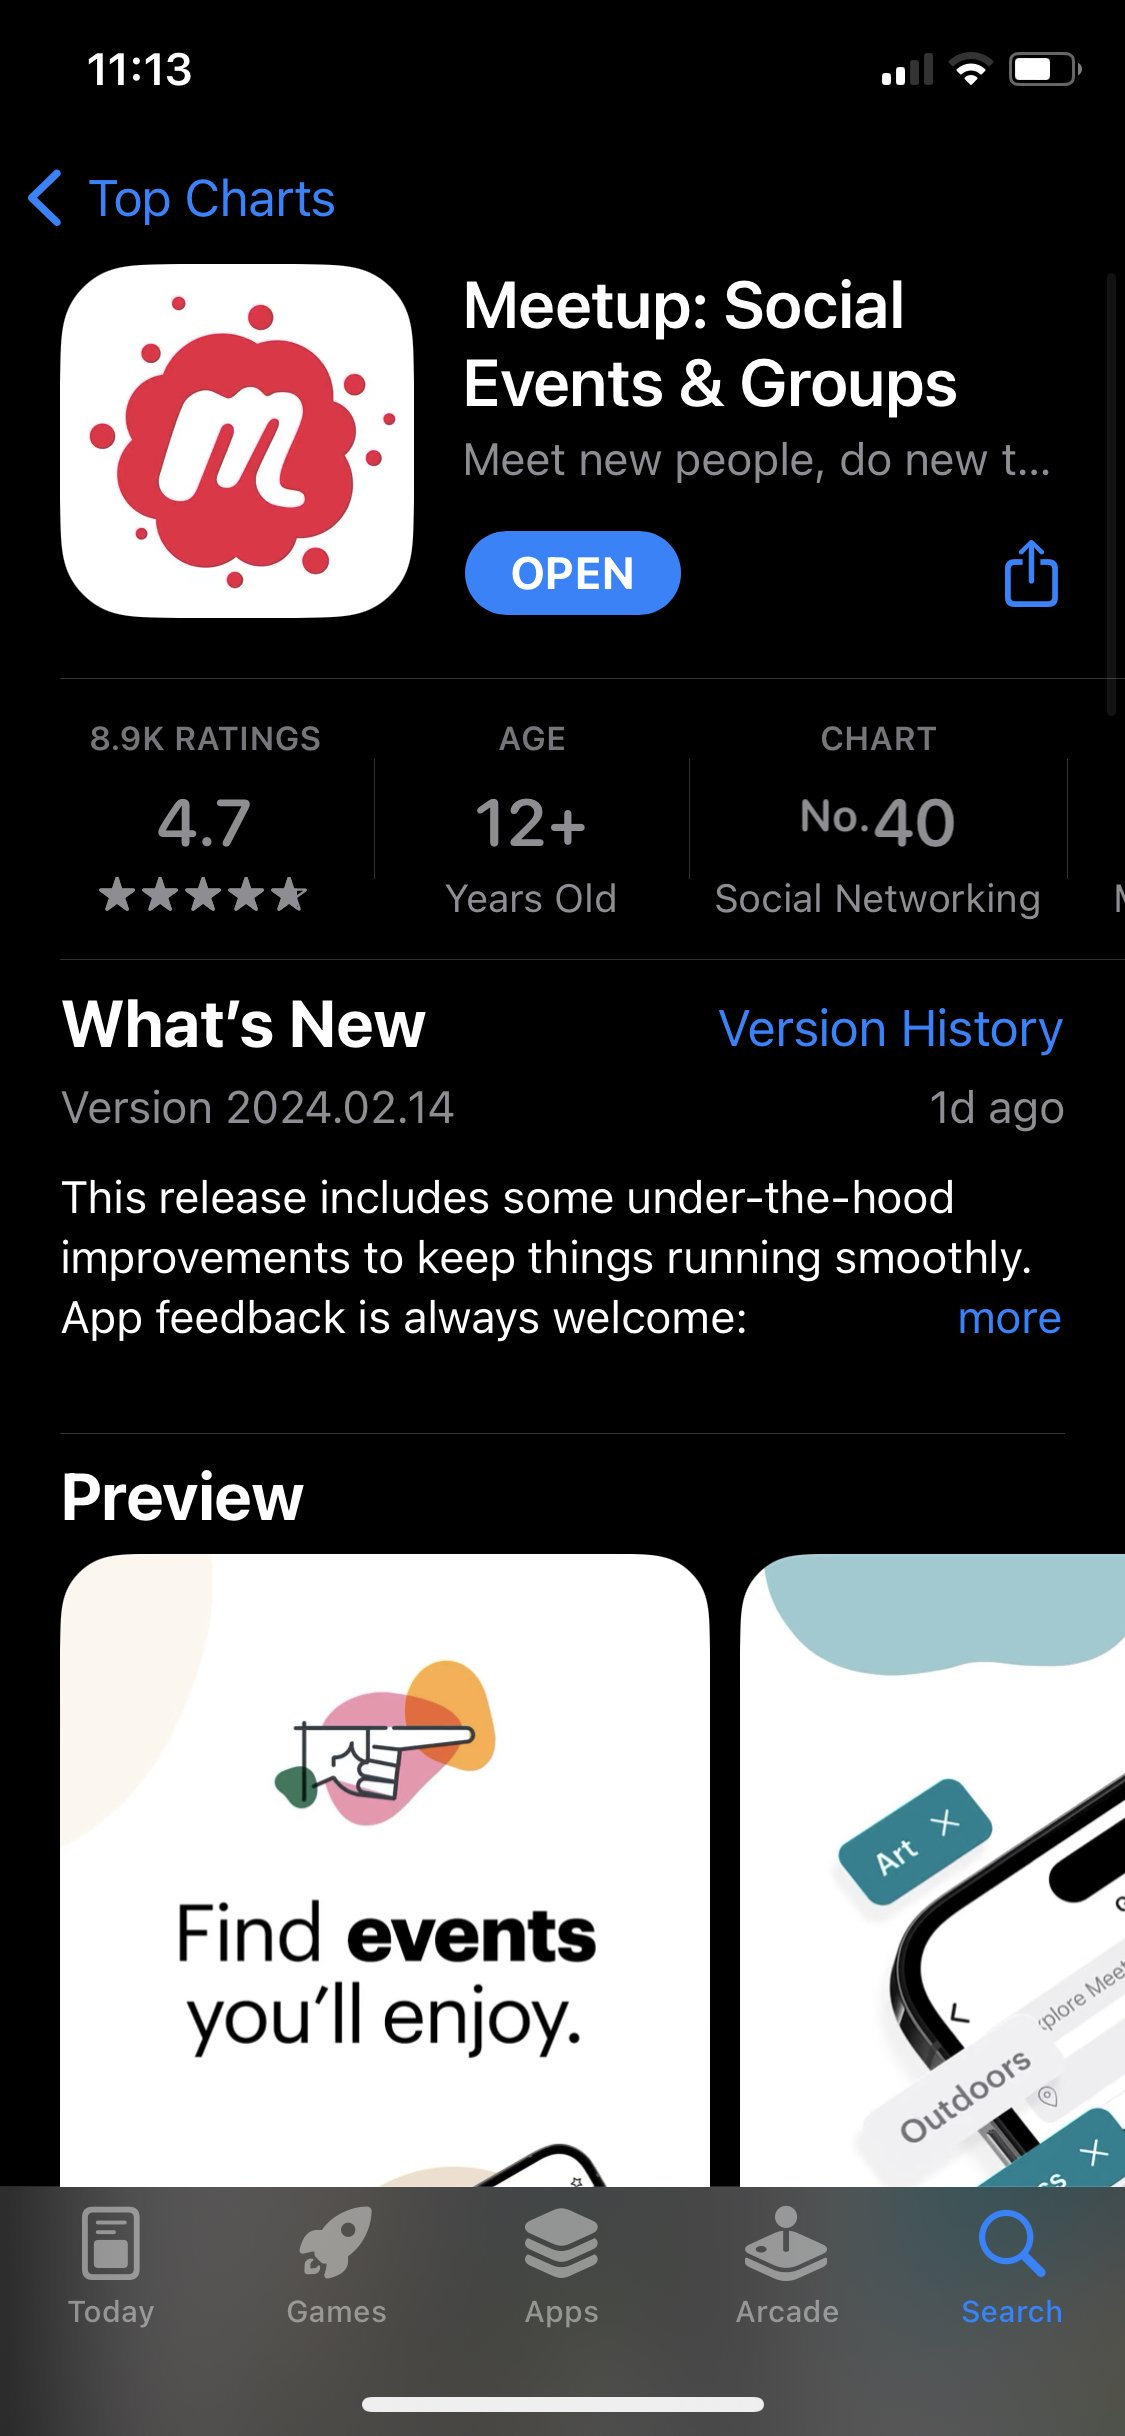
\includegraphics[cframe=black 2pt,width=0.3\linewidth]{images/estadodelarte/meetupappstore.jpeg}
  \caption{Meetup en la App Store}
  \label{fig:meetup_appstore}
\end{figure}
Actualmente, Meetup se cuenta entre las aplicaciones más populares tanto en iOS como en Android, 
ubicándose dentro del top 50 de aplicaciones en la categoría de redes sociales en la App Store de Appl\cite{REF12}. Meetup ha recaudado \verb|$|15.62 millones a lo largo de 9 rondas de financiación. 
Su última ronda de financiación fue el 11 de enero de 2024. La valoración de Meetup en noviembre de 2017 fue de entre \verb|$|156 y \verb|$|200 millones.\cite{REF11}

Entre las características de Meetup podemos encontrar las siguientes:

\begin{itemize}
  \item \textbf{Organización de grupos:} Los usuarios pueden formar y unirse a grupos basados en intereses comunes.
  \item \textbf{Planificación de eventos:} Los organizadores pueden planificar eventos dentro de su grupo, estableciendo 
  la fecha, la hora, el lugar y los detalles del evento.
  \item \textbf{RSVP para eventos:} Los usuarios pueden confirmar su asistencia a los eventos y ver quién más planea asistir.
  \item \textbf{Comunicación:} Los organizadores y los miembros del grupo pueden comunicarse a través de mensajes dentro de 
  la plataforma, permitiendo la coordinación y el intercambio de información.
  \item \textbf{Categorización de grupos:} Los grupos pueden ser categorizados en base a una variedad de intereses y 
  temas, facilitando a los usuarios encontrar grupos que coincidan con sus intereses.
  \item \textbf{Eventos locales y virtuales:} Meetup permite la organización de eventos tanto en persona como virtuales, 
  ofreciendo flexibilidad a los usuarios y organizadores.
  \item \textbf{Fotos y comentarios de eventos:} Después de un evento, los asistentes pueden publicar fotos y 
  comentarios, proporcionando un registro de la actividad del grupo y permitiendo a los miembros interactuar después del evento.
\end{itemize}
\begin{figure}[H]
        \centering
        
\includegraphics[width=0.3\linewidth]{images/Meetup_Logo.png}
        \caption{Logo de Meetup}
        \label{fig:meetup_logo}
    \end{figure}

\textbf{El modelo de negocio de Meetup}
Meetup opera bajo un modelo de negocio freemium, ofreciendo tanto una versión gratuita como una versión premium de la aplicación.
La versión de pago ofrece a participantes ventajas como ver quién está interesado en un evento, sin publicidad  y una insignia de verificado.
Para ser organizador de un grupo, se requiere una suscripción premium de un mayor costo que comienza desde los \verb|$|5.33 al mes.

\begin{figure}[H]
  \centering
  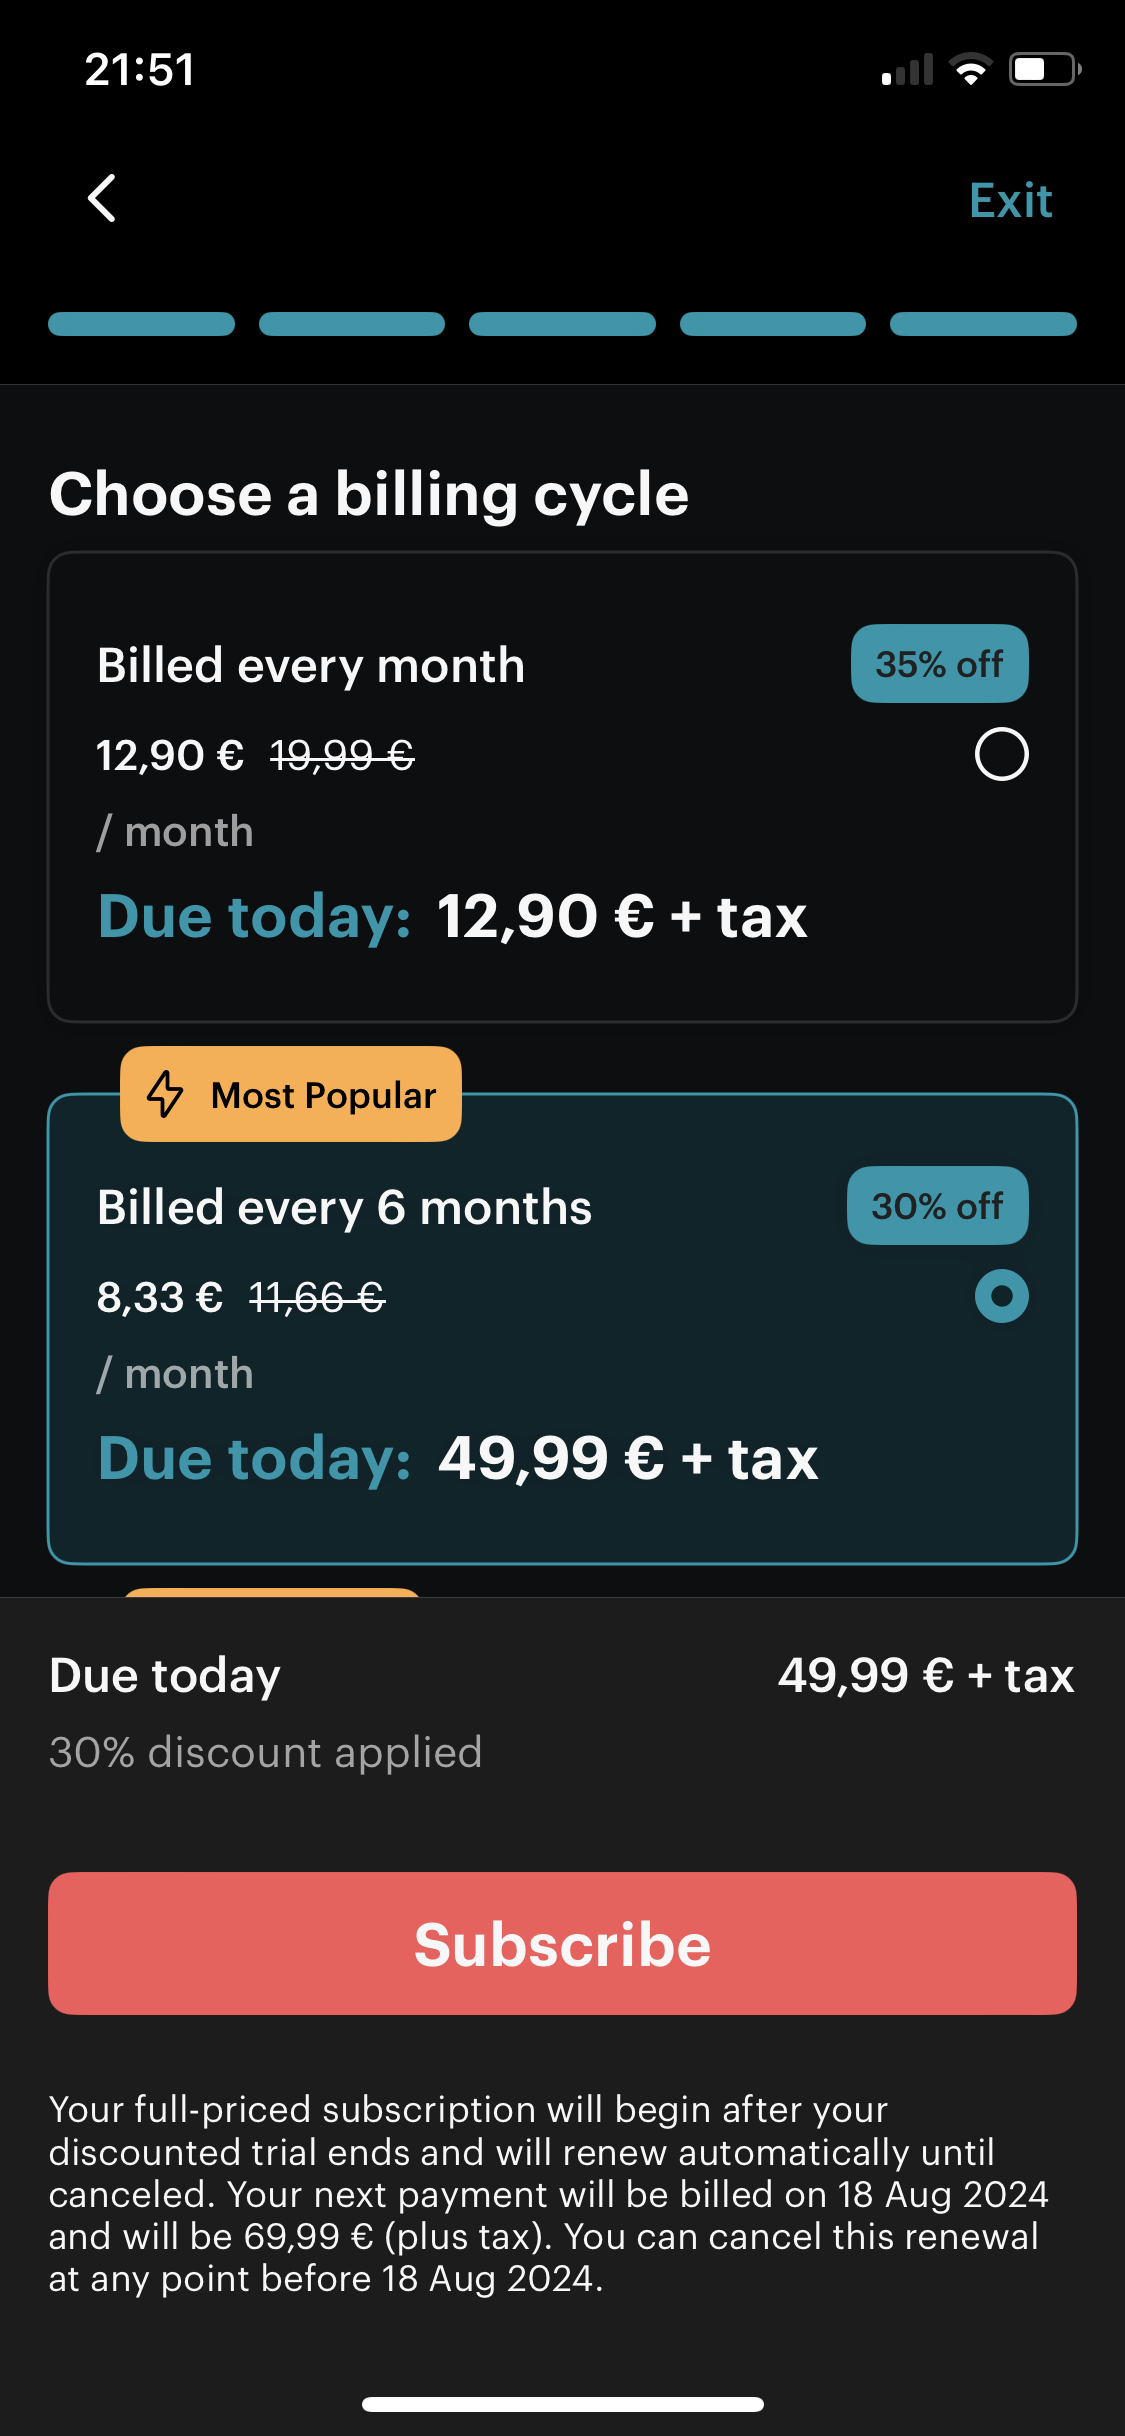
\includegraphics[cframe=black 2pt,width=0.3\linewidth]{images/estadodelarte/meetuporganizerprice.png}
  \caption{Meetup financials}
  \label{fig:meetup_financials}
\end{figure}

\textbf{El impacto de Meetup}

Meetup publicó su primer informe, denominado "State of Friendships"\cite{REF16}, donde revela estadísticas globales e insights sobre hobbies, 
intereses y la formación de nuevas amistades.
Entre las conclusiones podemos destacar:
\begin{itemize}
  \item \textbf{La importancia de la amistad:} Hacer amigos es el principal motivo por el que las personas se unen a Meetup.
  \item \textbf{Los países más activos:} Los países con mayor actividad en Meetup son Estados Unidos, Australia, Singapur seguido de Canadá y Irlanda.
  \item \textbf{Palabras clave:} Las palabras clave más populares en Meetup son "senderismo", "amigos", "social", "fotografía" y "club de lectura".
\subsection{Strava}

Strava es mucho más que una aplicación para el seguimiento de la actividad física; ha logrado cultivar una comunidad global apasionada de corredores. 
Sus características sociales juegan un papel crucial en atraer, comprometer y retener a su amplia base de usuarios.

Fundada en 2009, Strava originalmente atendía principalmente a ciclistas. 
Sin embargo, correr rápidamente se convirtió en un enfoque central, aceptando deportes como natación, senderismo, etc.
La aplicación se posicionó de manera única para aprovechar los conceptos de redes sociales dentro del contexto de 
deportistas  en busca de conexión, motivación y competencia amistosa.

\textbf{Cómo Strava Reúne a los Corredores: El Poder de lo Social}

\textit{Clubes:} Los clubes de Strava sirven como comunidades de corredores virtuales centradas en ubicaciones específicas, intereses 
o marcas. Proporcionan un espacio para discusiones en grupo, carreras organizadas y metas compartidas.

\begin{figure}[H]
  \centering
  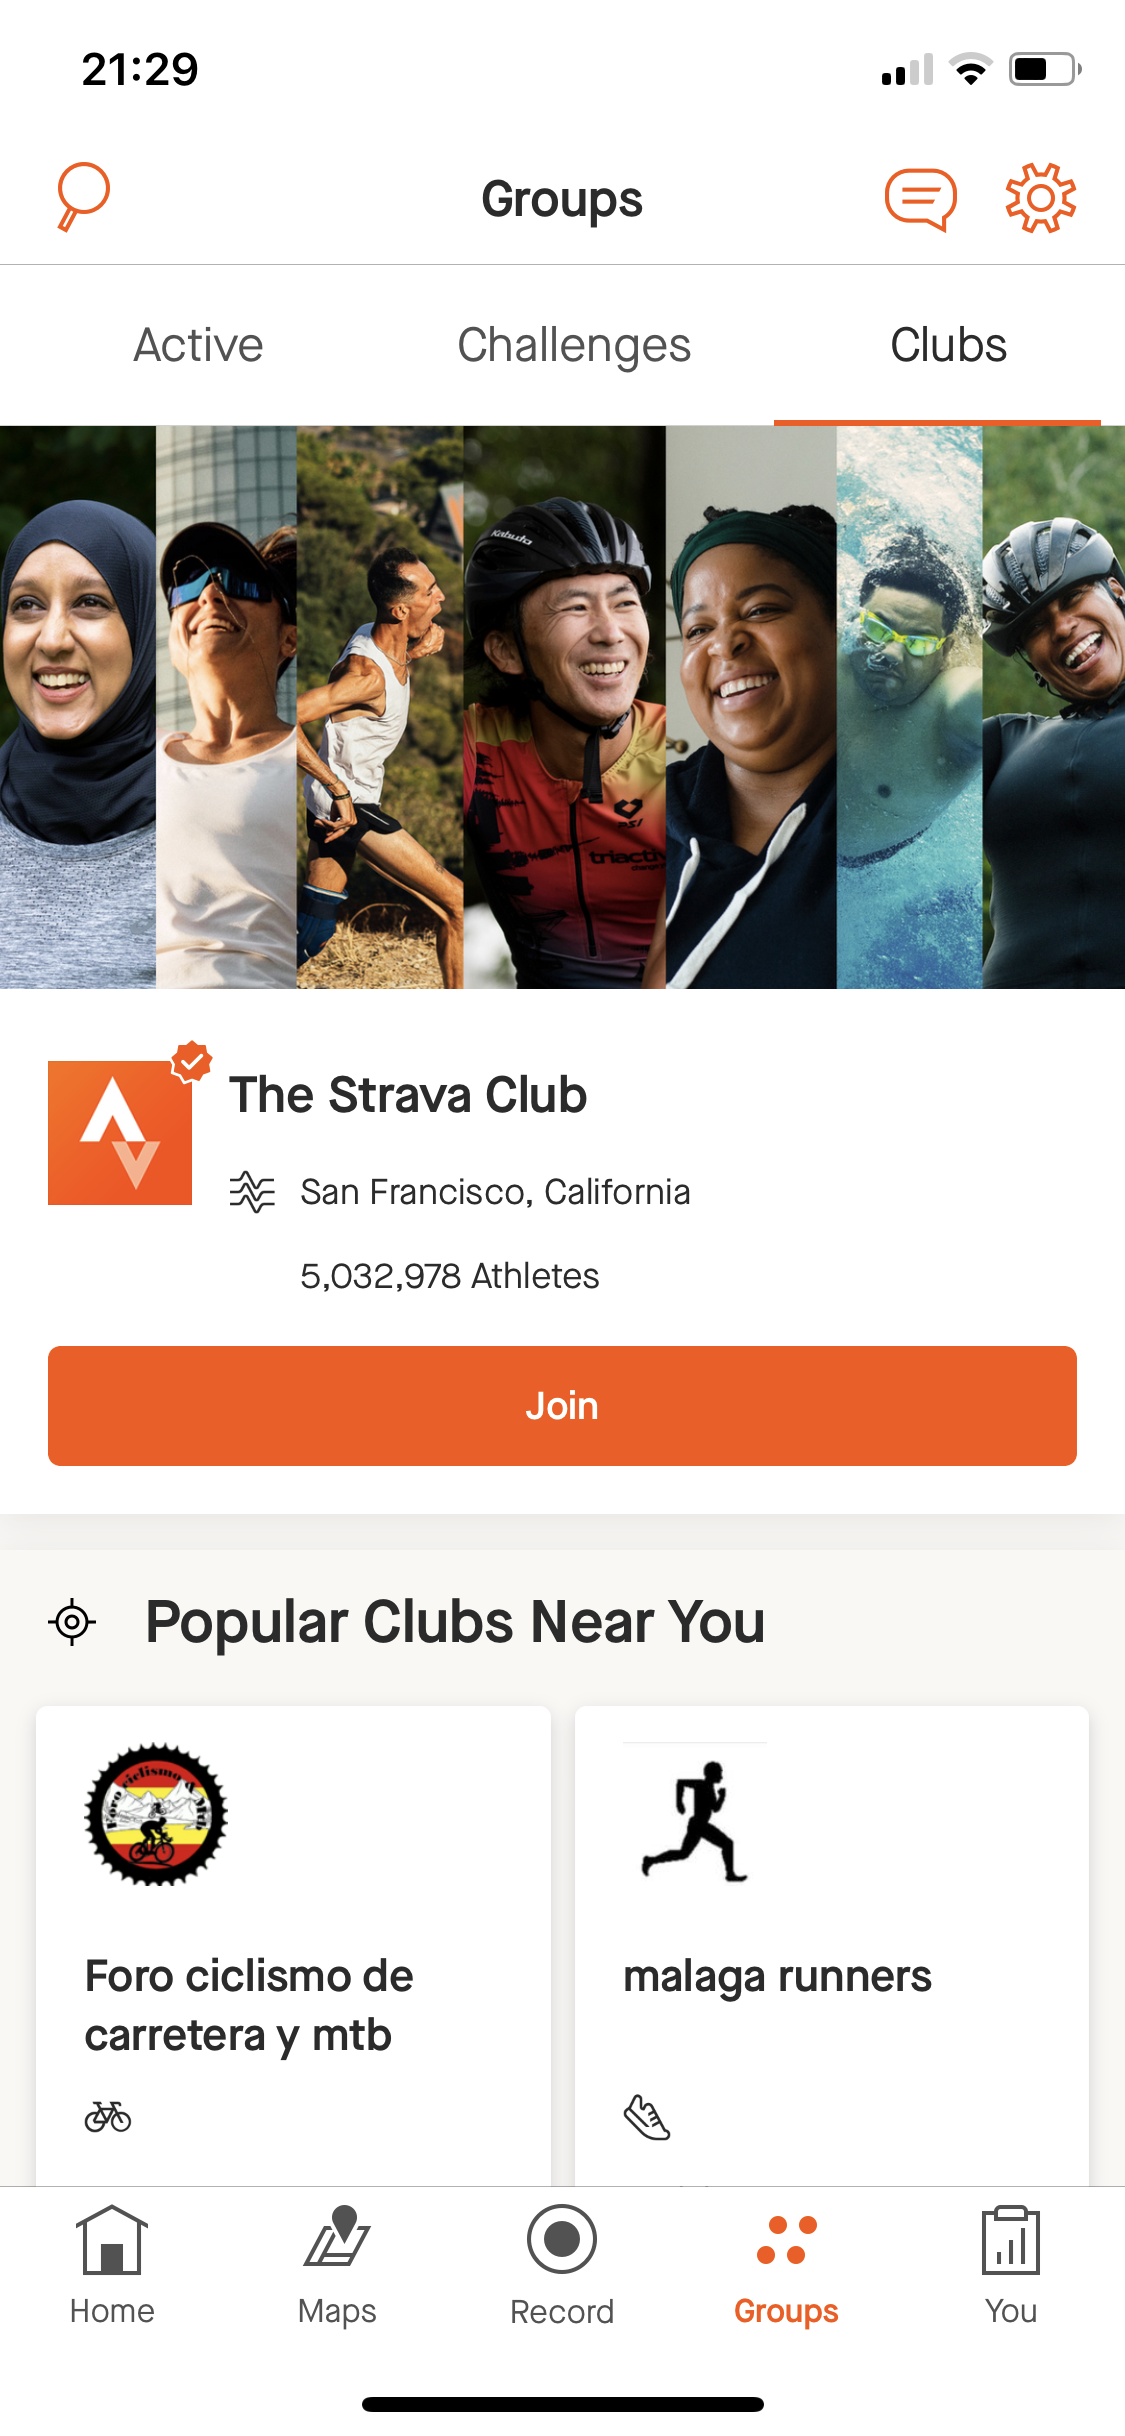
\includegraphics[cframe=black 2pt,width=0.3\linewidth]{images/estadodelarte/stravaclubs.png}
  \caption{Clubes de Strava}
  \label{fig:strava_clubs}
\end{figure}

\item \textbf{Posts, Kudos y Comentarios}: Strava permite a corredores de todos los niveles compartir datos de entrenamiento, 
rutas y fotos, creando un sentido de experiencia compartida y una plataforma para celebrar logros, incluso entre corredores de 
todo el mundo. Características simples como "kudos" (similares a me gusta) y comentarios generan refuerzo positivo y crean una 
atmósfera en línea de apoyo. Estas interacciones rápidas aumentan la motivación y construyen conexiones.

\begin{figure}[H]
  \centering
  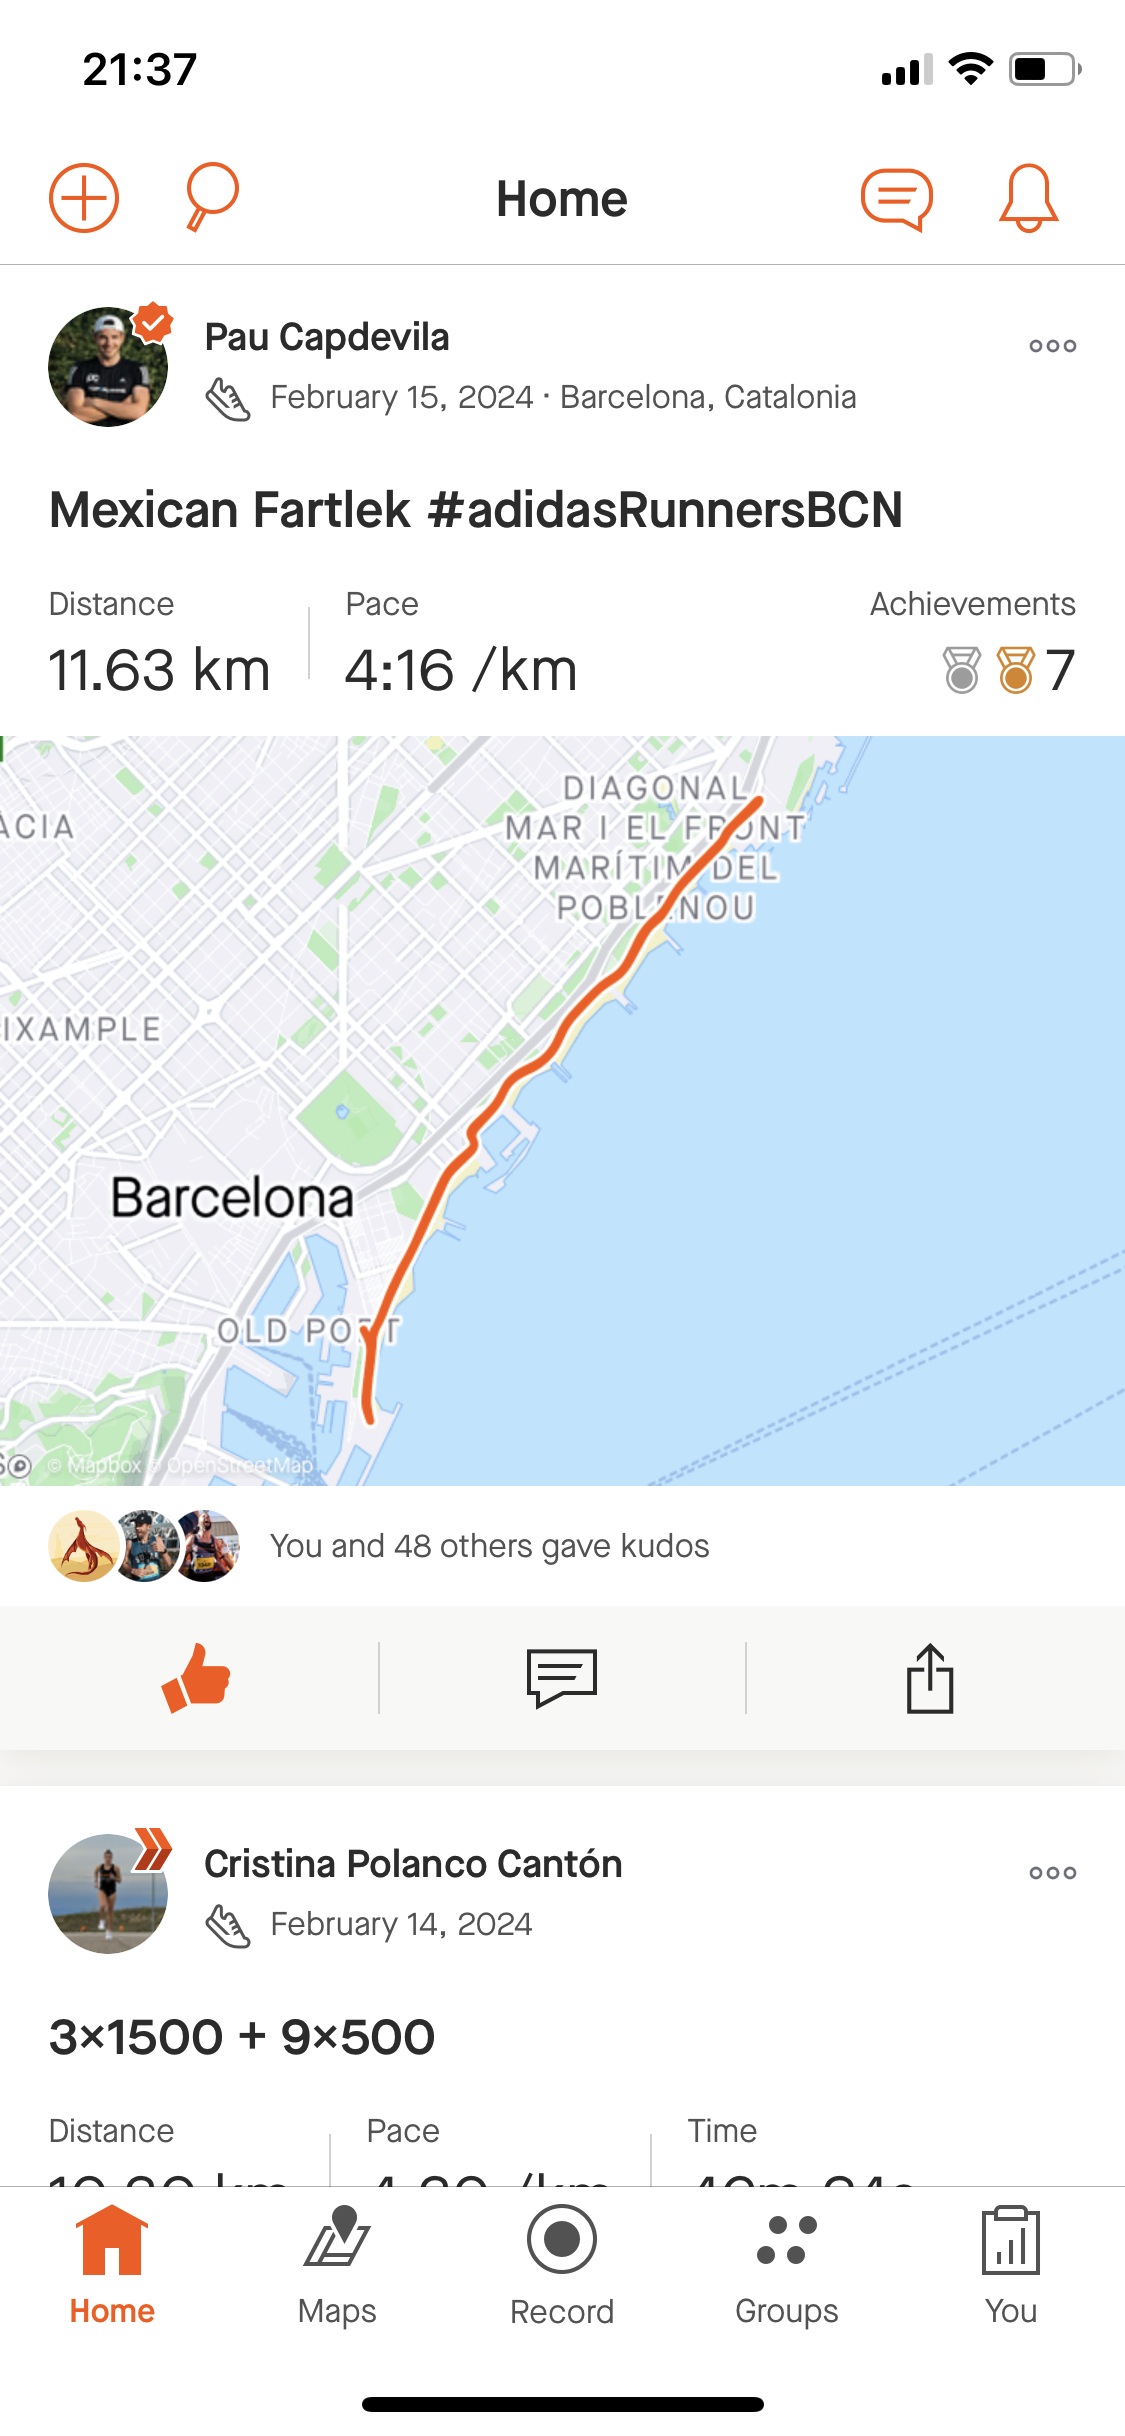
\includegraphics[cframe=black 2pt,width=0.3\linewidth]{images/estadodelarte/stravaposts.jpeg}
  \caption{Posts de Strava}
  \label{fig:strava_posts}
\end{figure}


\item \textbf{Segmentos y Tablas de Clasificación:} Los segmentos de Strava – porciones designadas de carreras o paseos – convierten cada 
sendero o camino en una competencia. Las tablas de clasificación fomentan una rivalidad, empujando a los corredores a esforzarse por mejores personales y una mayor colocación.

\item \textbf{Desafíos:} Los desafíos mensuales y patrocinados por marcas dan a los corredores objetivos para entrenar y construir un 
sentido de camaradería con otros comprometidos en el mismo desafío.

\begin{figure}[H]
  \centering
  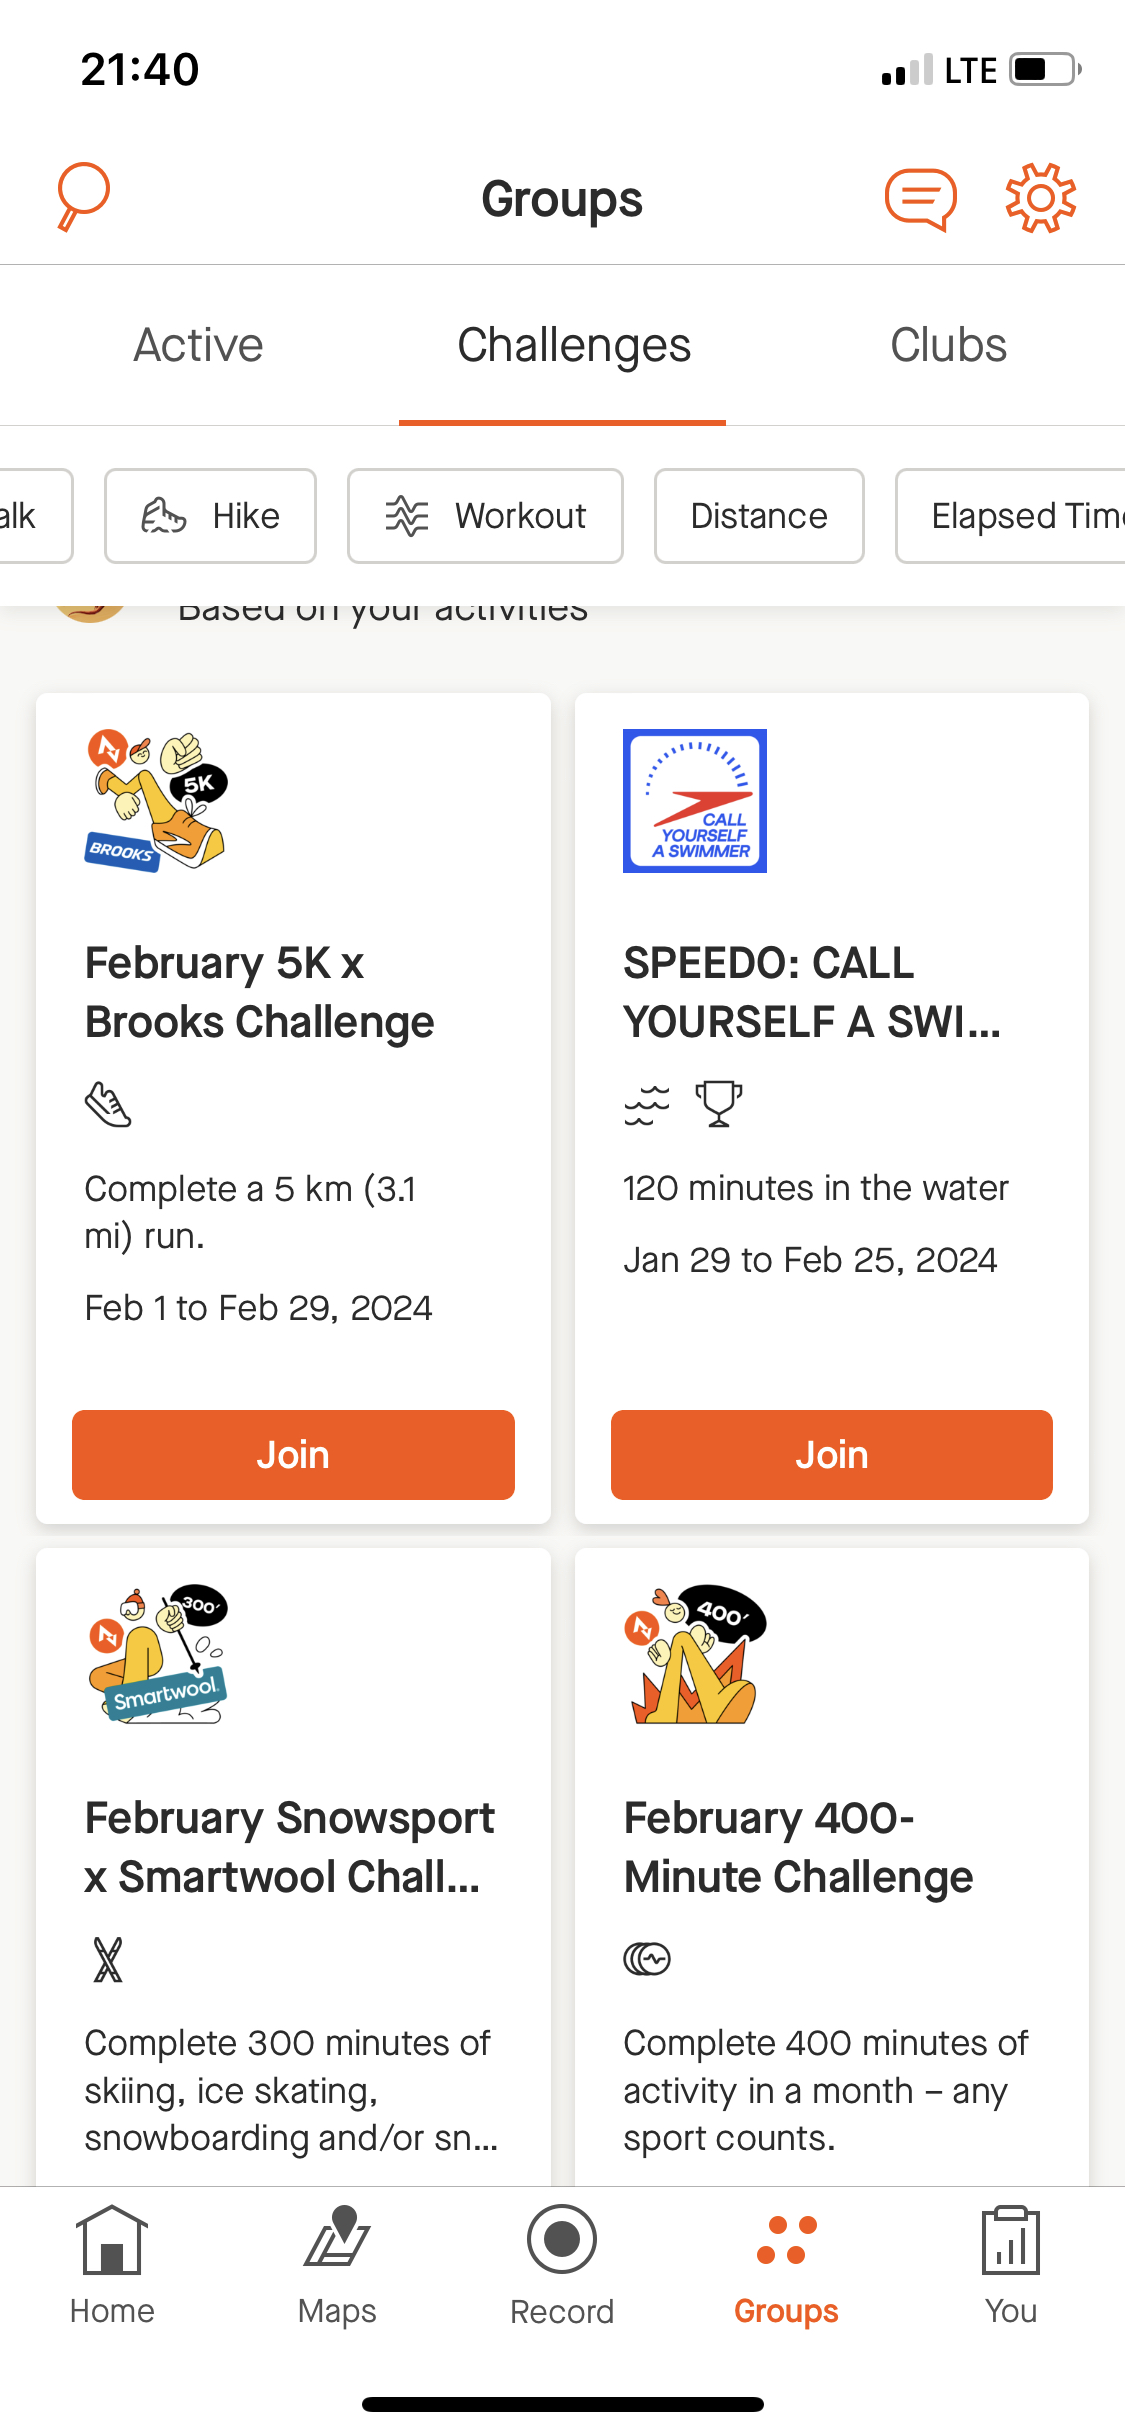
\includegraphics[cframe=black 2pt,width=0.3\linewidth]{images/estadodelarte/stravachallenges.jpeg}
  \caption{Desafíos de Strava}
  \label{fig:strava_challenges}
\end{figure}


\textbf{Factores Adicionales de Éxito}

\textit{Compatibilidad:} Strava se integra fácilmente con dispositivos GPS populares y relojes inteligentes, aumentando su atractivo 
y simplificando la entrada de datos.

\textit{Modelo Freemium:} Aunque ofrece características premium, los elementos sociales centrales están disponibles de forma 
gratuita, facilitando la adopción y el crecimiento de la base de usuarios.

\textit{Énfasis en lo Visual:} Los mapas, gráficos de elevación y fotos hacen que los feeds de actividad sean atractivos, 
atrayendo a los usuarios de vuelta a la aplicación.

\textbf{Conclusión}

La potente mezcla de elementos sociales de Strava crea un entorno convincente y motivador para los corredores. Entiende la 
naturaleza social de correr y proporciona formas significativas para que los corredores se conecten, se apoyen mutuamente y celebren logros, todo mientras impulsan el uso de la aplicación.


\subsection{Amigos Social}
Amigos Social es una plataforma social única que enfatiza las conexiones en la vida real y las experiencias compartidas de 
manera espontánea. A diferencia de las aplicaciones de redes sociales tradicionales, que a menudo se centran en perfiles en línea y contenido curado, 
Amigos Social busca cerrar la brecha entre las interacciones en línea y los encuentros en persona.

El concepto detrás de Amigos Social surgió en respuesta a un creciente sentido de aislamiento y una falta de compromiso social 
satisfactorio en nuestro mundo cada vez más digital. Amigos Social comenzó como una plataforma de nicho pero ha visto un crecimiento constante en popularidad, particularmente entre las demografías más jóvenes.


\textbf{Problemas Principales Abordados}

Amigos Social aborda los siguientes problemas centrales dentro del panorama de las redes sociales:

\item \textbf{Aislamiento y Soledad:} La aplicación crea un camino para la conexión significativa, especialmente para aquellos que luchan por encontrar individuos afines en su entorno inmediato.
\item \textbf{Torpeza Social:} Minimiza la torpeza de iniciar interacciones sociales al ofrecer una estructura y actividades compartidas para romper el hielo.
\item \textbf{Aburrimiento y Estancamiento:} La naturaleza espontánea de la aplicación ayuda a los usuarios a salir de las rutinas y descubrir nuevas experiencias.
\item \textbf{Esfera Social Limitada:} Amigos Social promueve la expansión fácil del círculo social de uno, permitiendo a los usuarios conectarse basados en intereses compartidos y ubicación.

\textbf{Características Destacadas}

Las características sobresalientes de Amigos Social incluyen:

\item \textbf{Creación y Descubrimiento de Eventos en Tiempo Real:} Los usuarios pueden generar rápidamente eventos sociales con temas variados (caminatas, encuentros para tomar café, fiestas, etc.) abiertos para que otros se unan en su área.
Dentro de la creación de eventos social podemos destacar características como por ejemplo la obligación de contribuir a un evento, es decir que el organizador 
puede obligar a los asistentes a contribuir con una pequeña cantidad de dinero para asergurar el compromiso de los asistentes.
\begin{figure}[H]
  \centering
  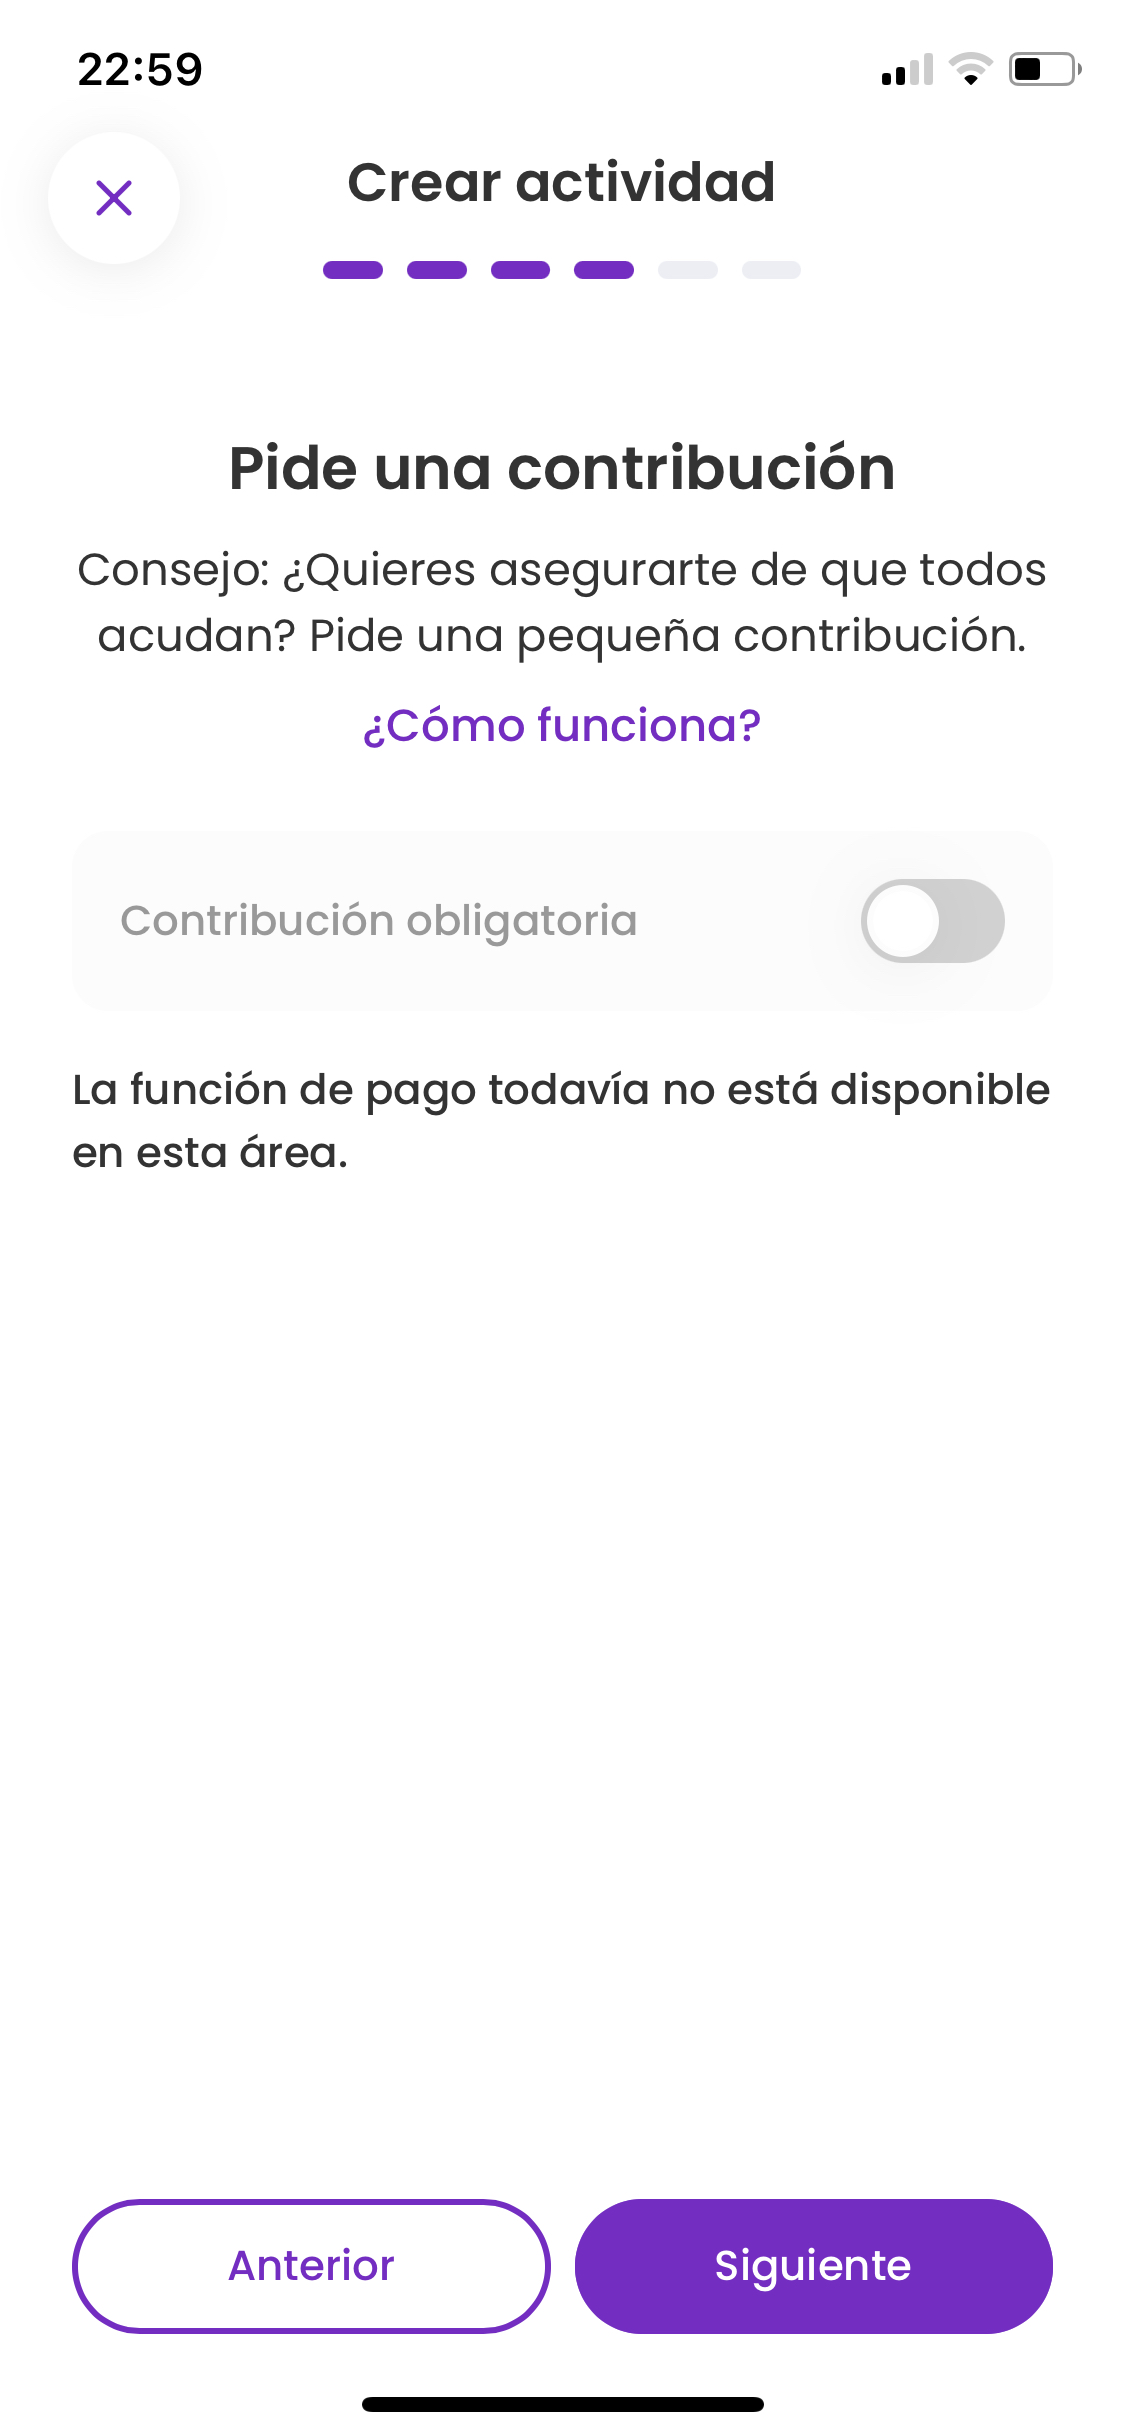
\includegraphics[cframe=black 2pt,width=0.3\linewidth]{images/estadodelarte/amigossocialcontribucion.jpeg}
  \caption{Obligar contribución en Amigos Social}
  \label{fig:amigosocial_contribucion}
\end{figure}
También la app ofrece distintos parámetros para la creación de eventos, como por ejemplo la posibilidad de establecer un límite de asistentes.
\begin{figure}[H]
  \centering
  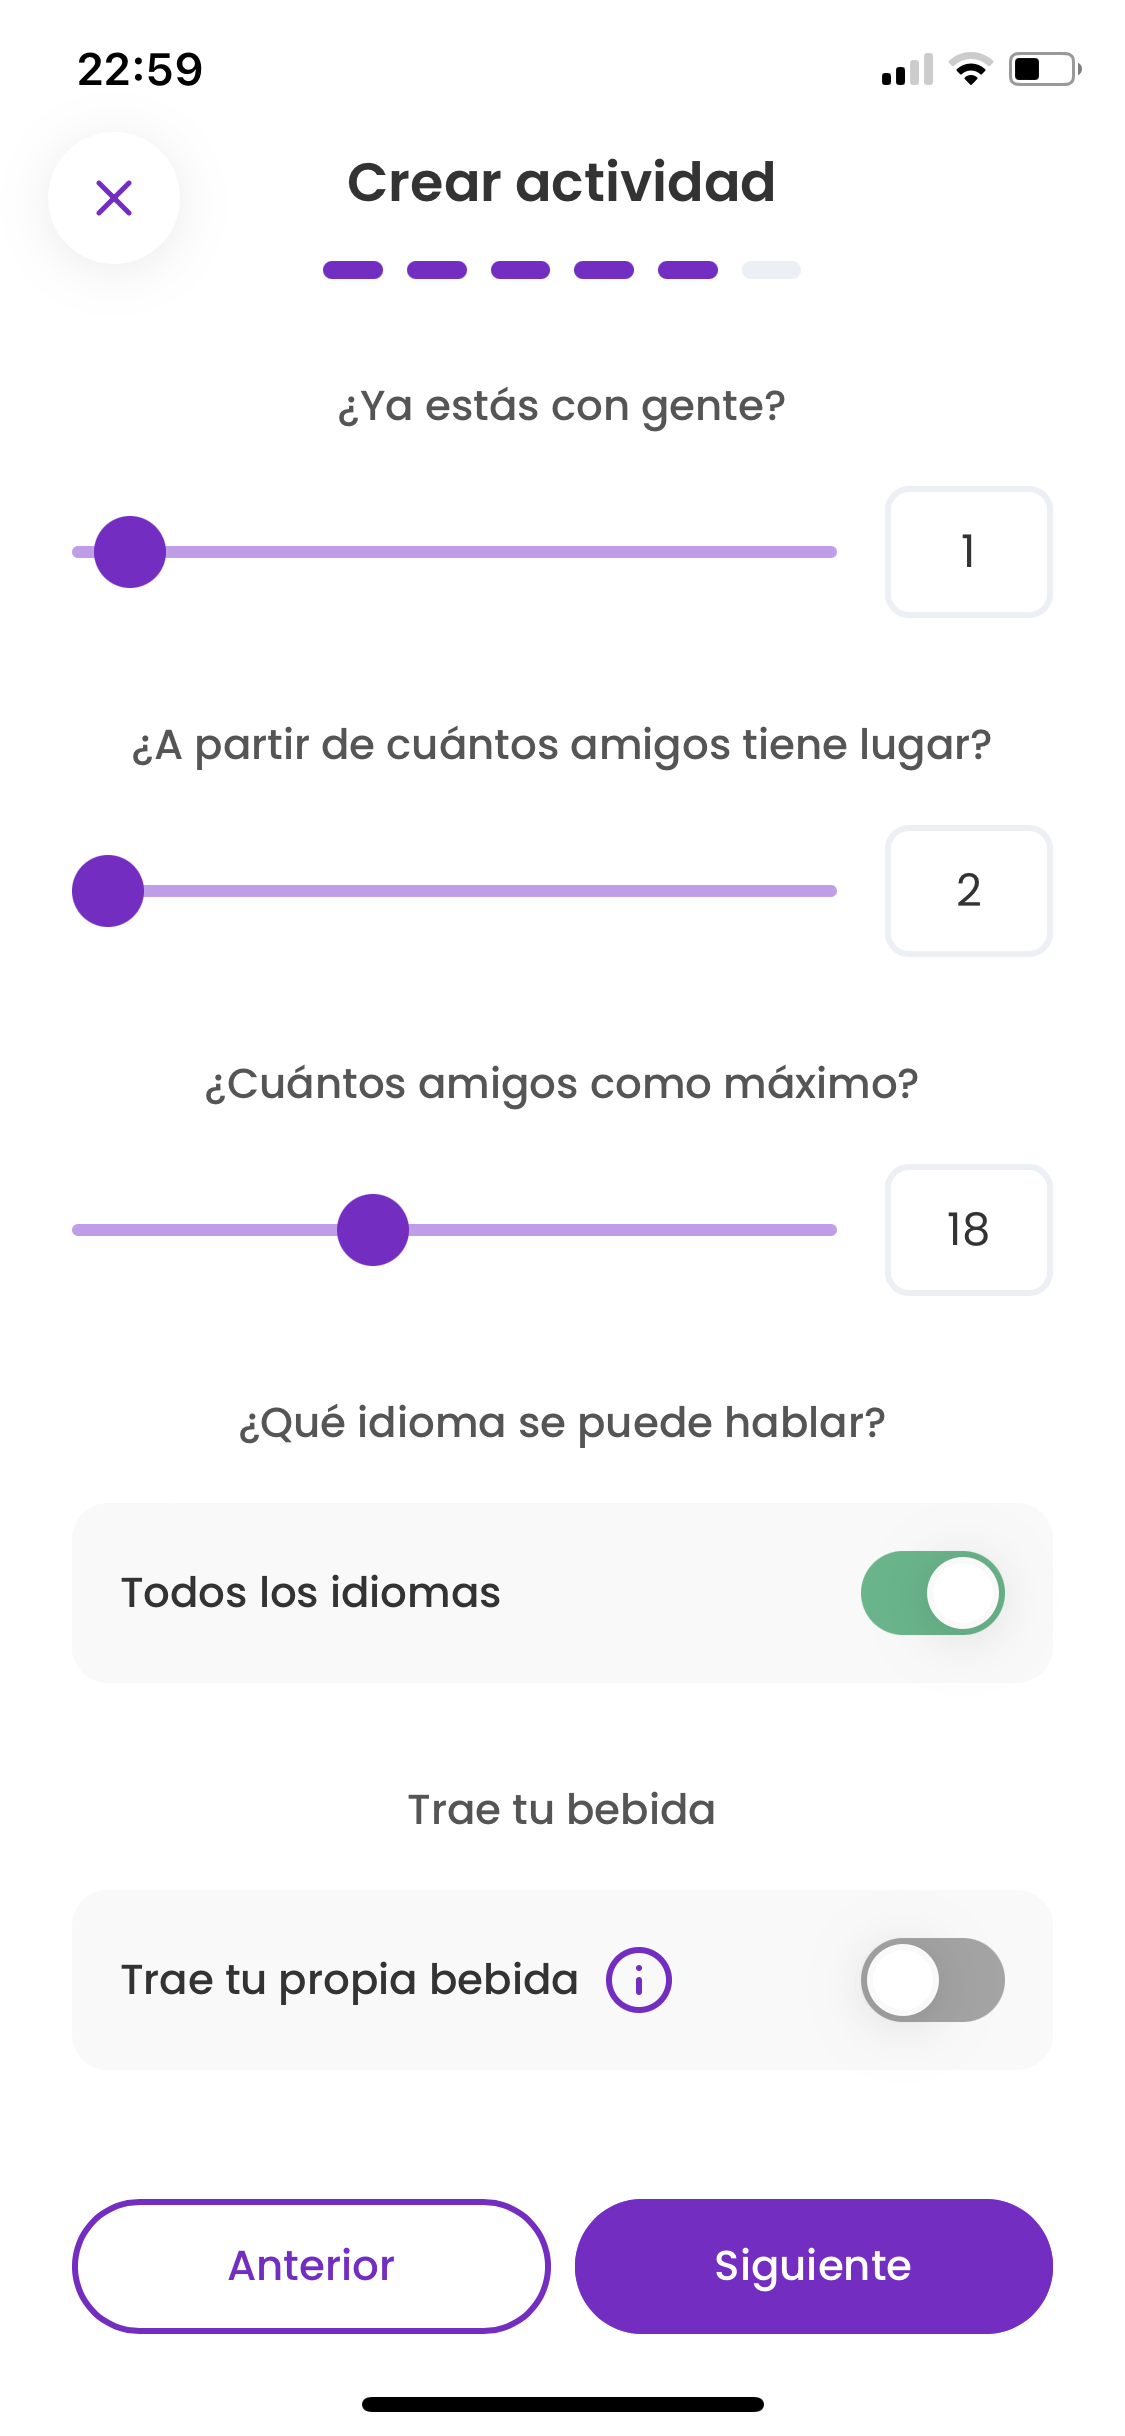
\includegraphics[cframe=black 2pt,width=0.3\linewidth]{images/estadodelarte/amigossocialasistentes.jpeg}
  \caption{Límite de asistentes en Amigos Social}
  \label{fig:amigosocial_asistentes}
\end{figure}
\item \textbf{Emparejamiento Basado en Proximidad:} Su interfaz de búsqueda es un mapa que resalta eventos que ocurren cerca y los distintos intereses de personas, es decir que los usuarios pueden 
indicar en que tipo de actividades están dispuestos a participar.
\begin{figure}[H]
  \centering
  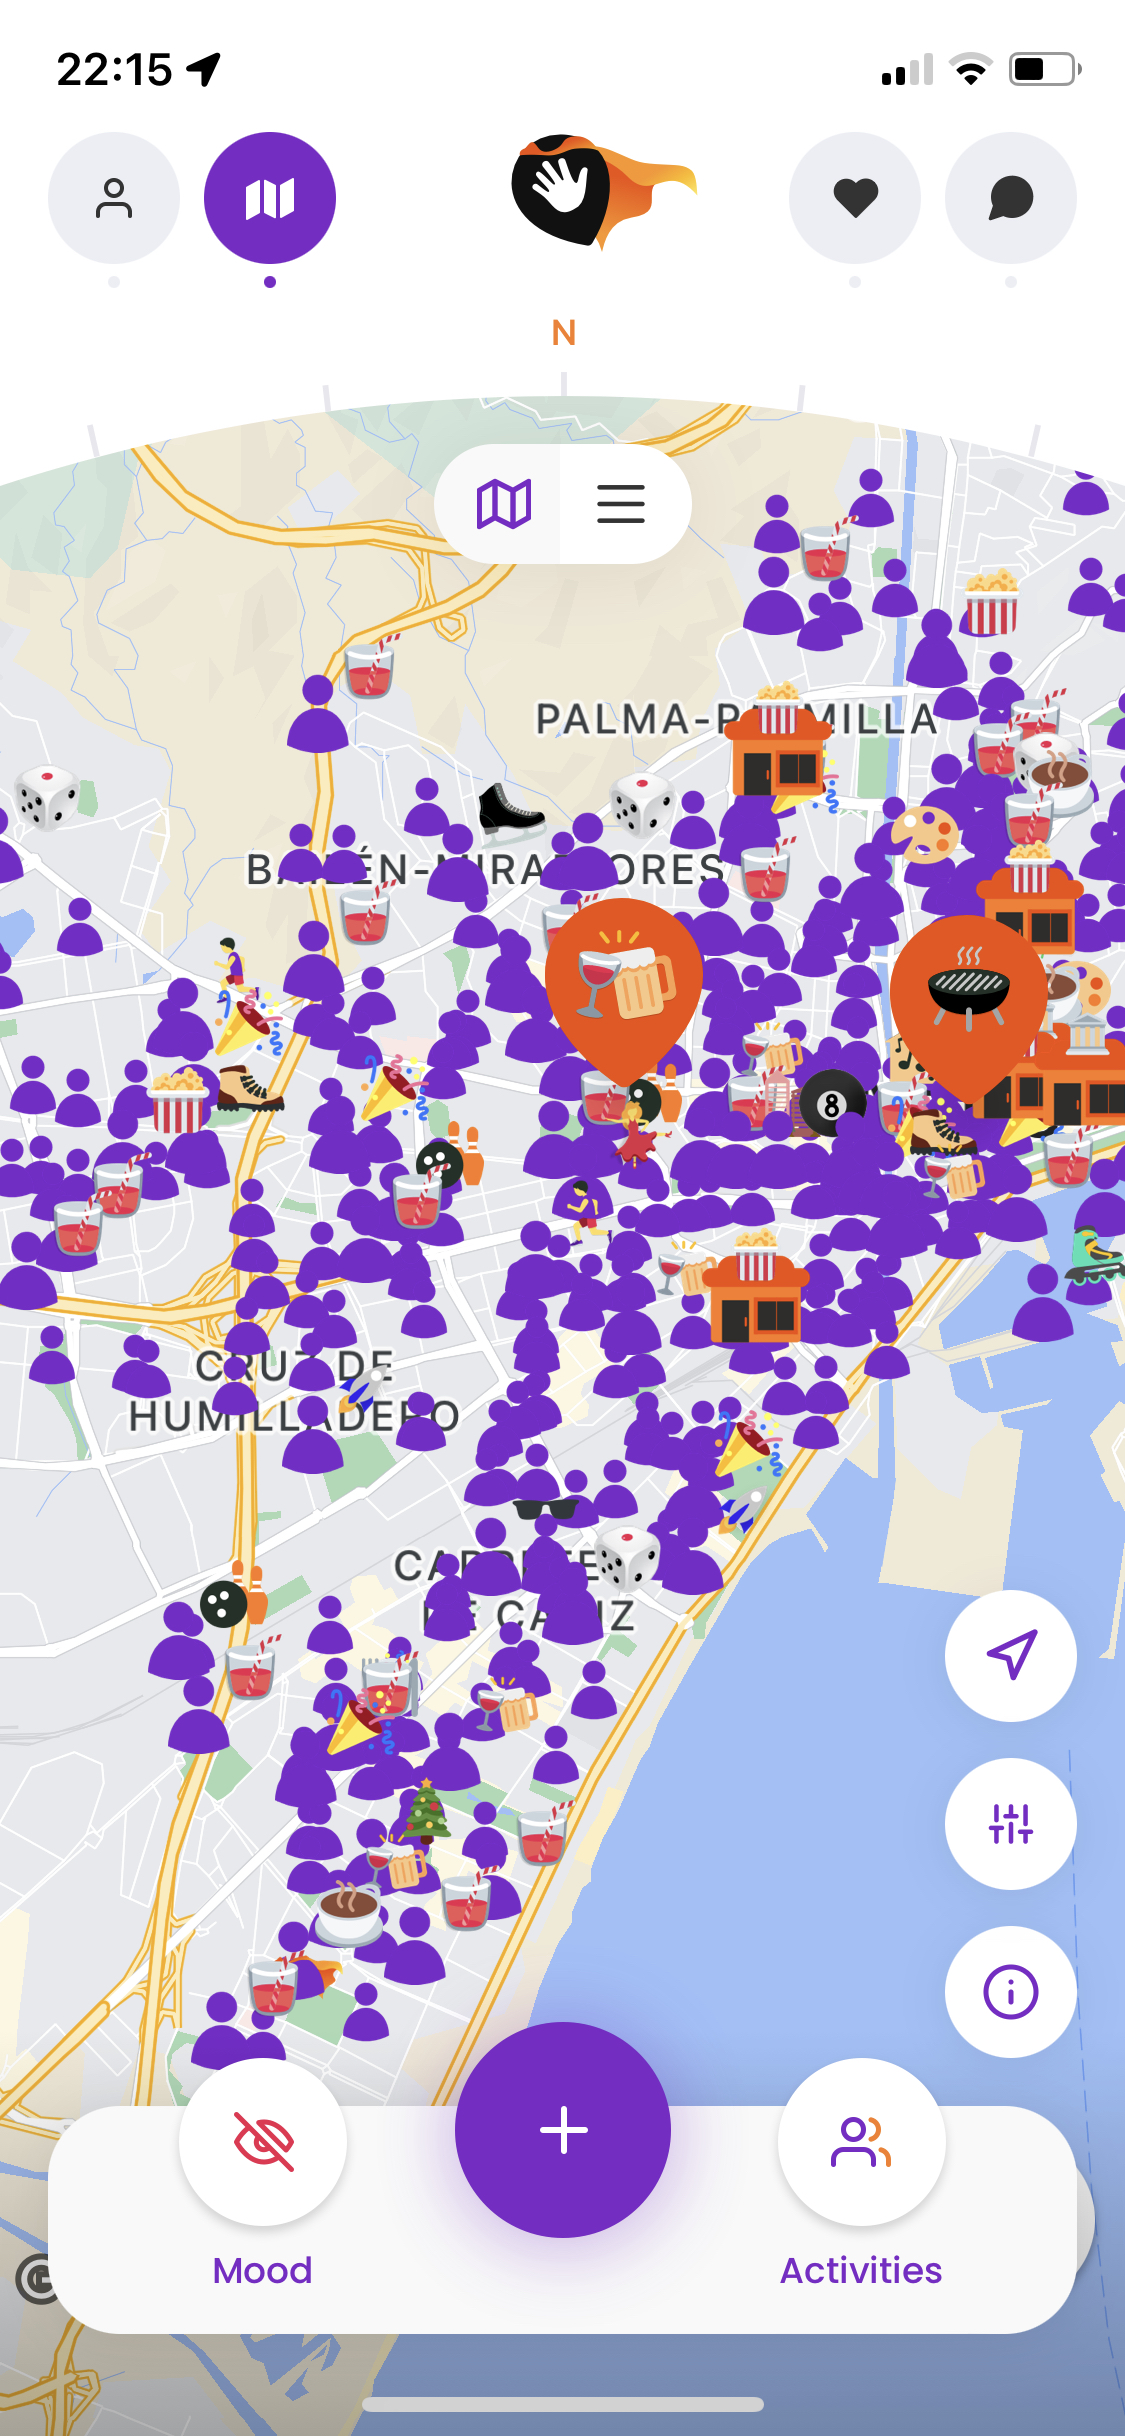
\includegraphics[cframe=black 2pt,width=0.3\linewidth]{images/estadodelarte/amigossocialmap.jpeg}
  \caption{Mapa de Amigos Social}
  \label{fig:amigosocial_map}
\end{figure}
\item \textit{Intereses Diversos:} La aplicación apoya una amplia gama de intereses y actividades, asegurando que haya algo para casi todos.
\begin{figure}[H]
  \centering
  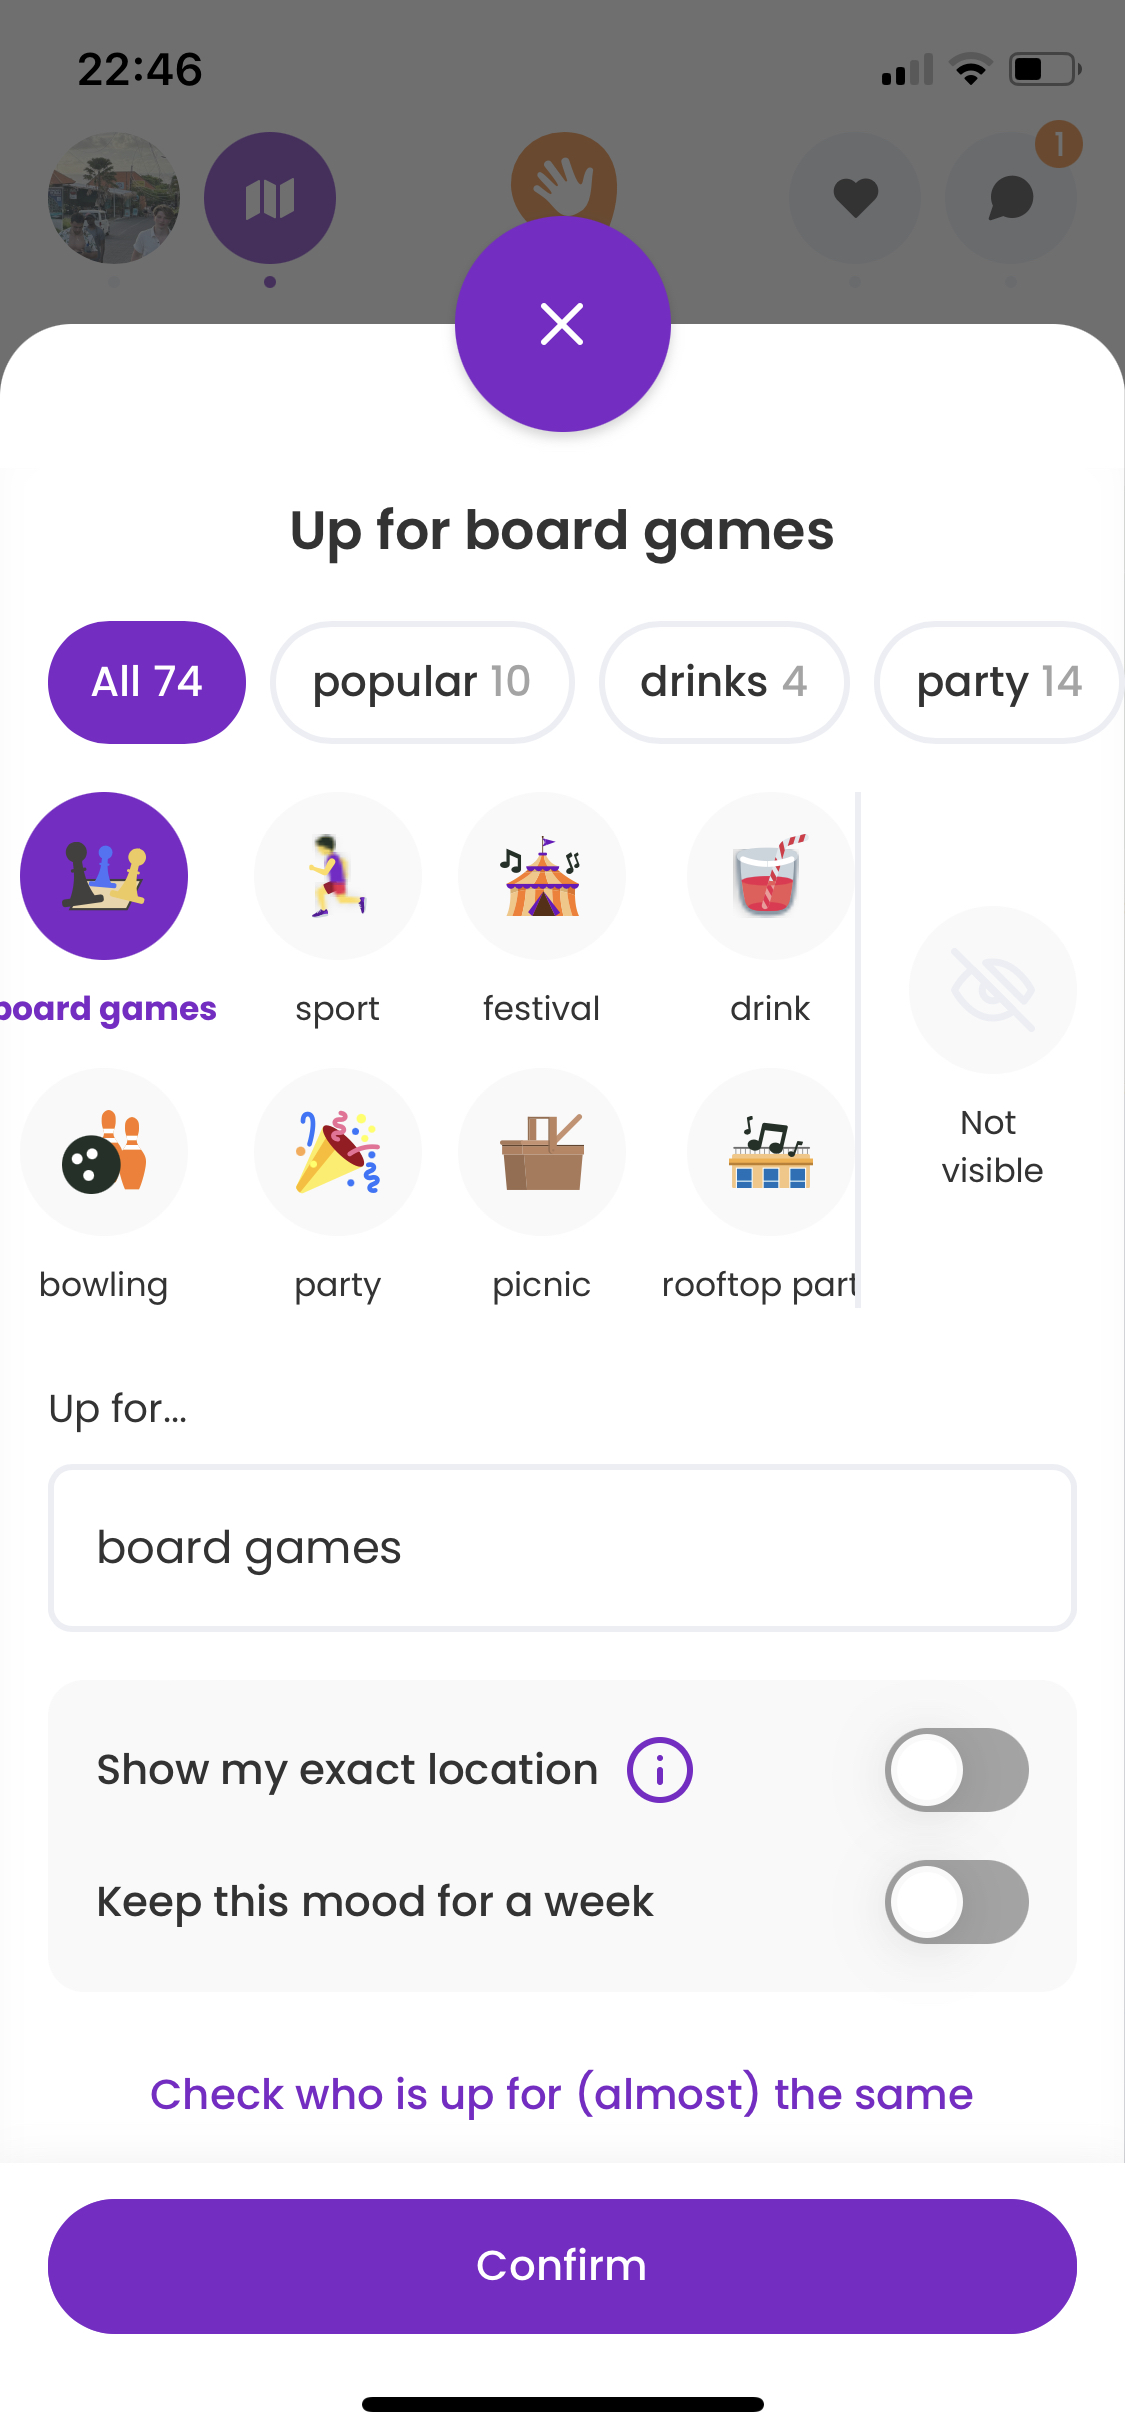
\includegraphics[cframe=black 2pt,width=0.3\linewidth]{images/estadodelarte/amigossocialinterests.jpeg}
  \caption{Intereses de Amigos Social}
  \label{fig:amigosocial_interests}
\end{figure}

\item \textit{Énfasis en la Espontaneidad:} Con eventos siendo creados y unidos en tiempo real, Amigos Social atiende al deseo de conexión social bajo demanda.

\textbf{Modelo de Negocio}
La app en su mayor parte es gratis, simplemente ofrece una suscripción premium que aumenta tu visibilidad a través de una insignia además de funciones exclusivas.
Pero no ofrece nada característico y diferenciador que haga que el usuario este dispuesto a pagar por ello, por eso el precio es de \verb|$|2.99 al mes.

\begin{figure}[H]
  \centering
  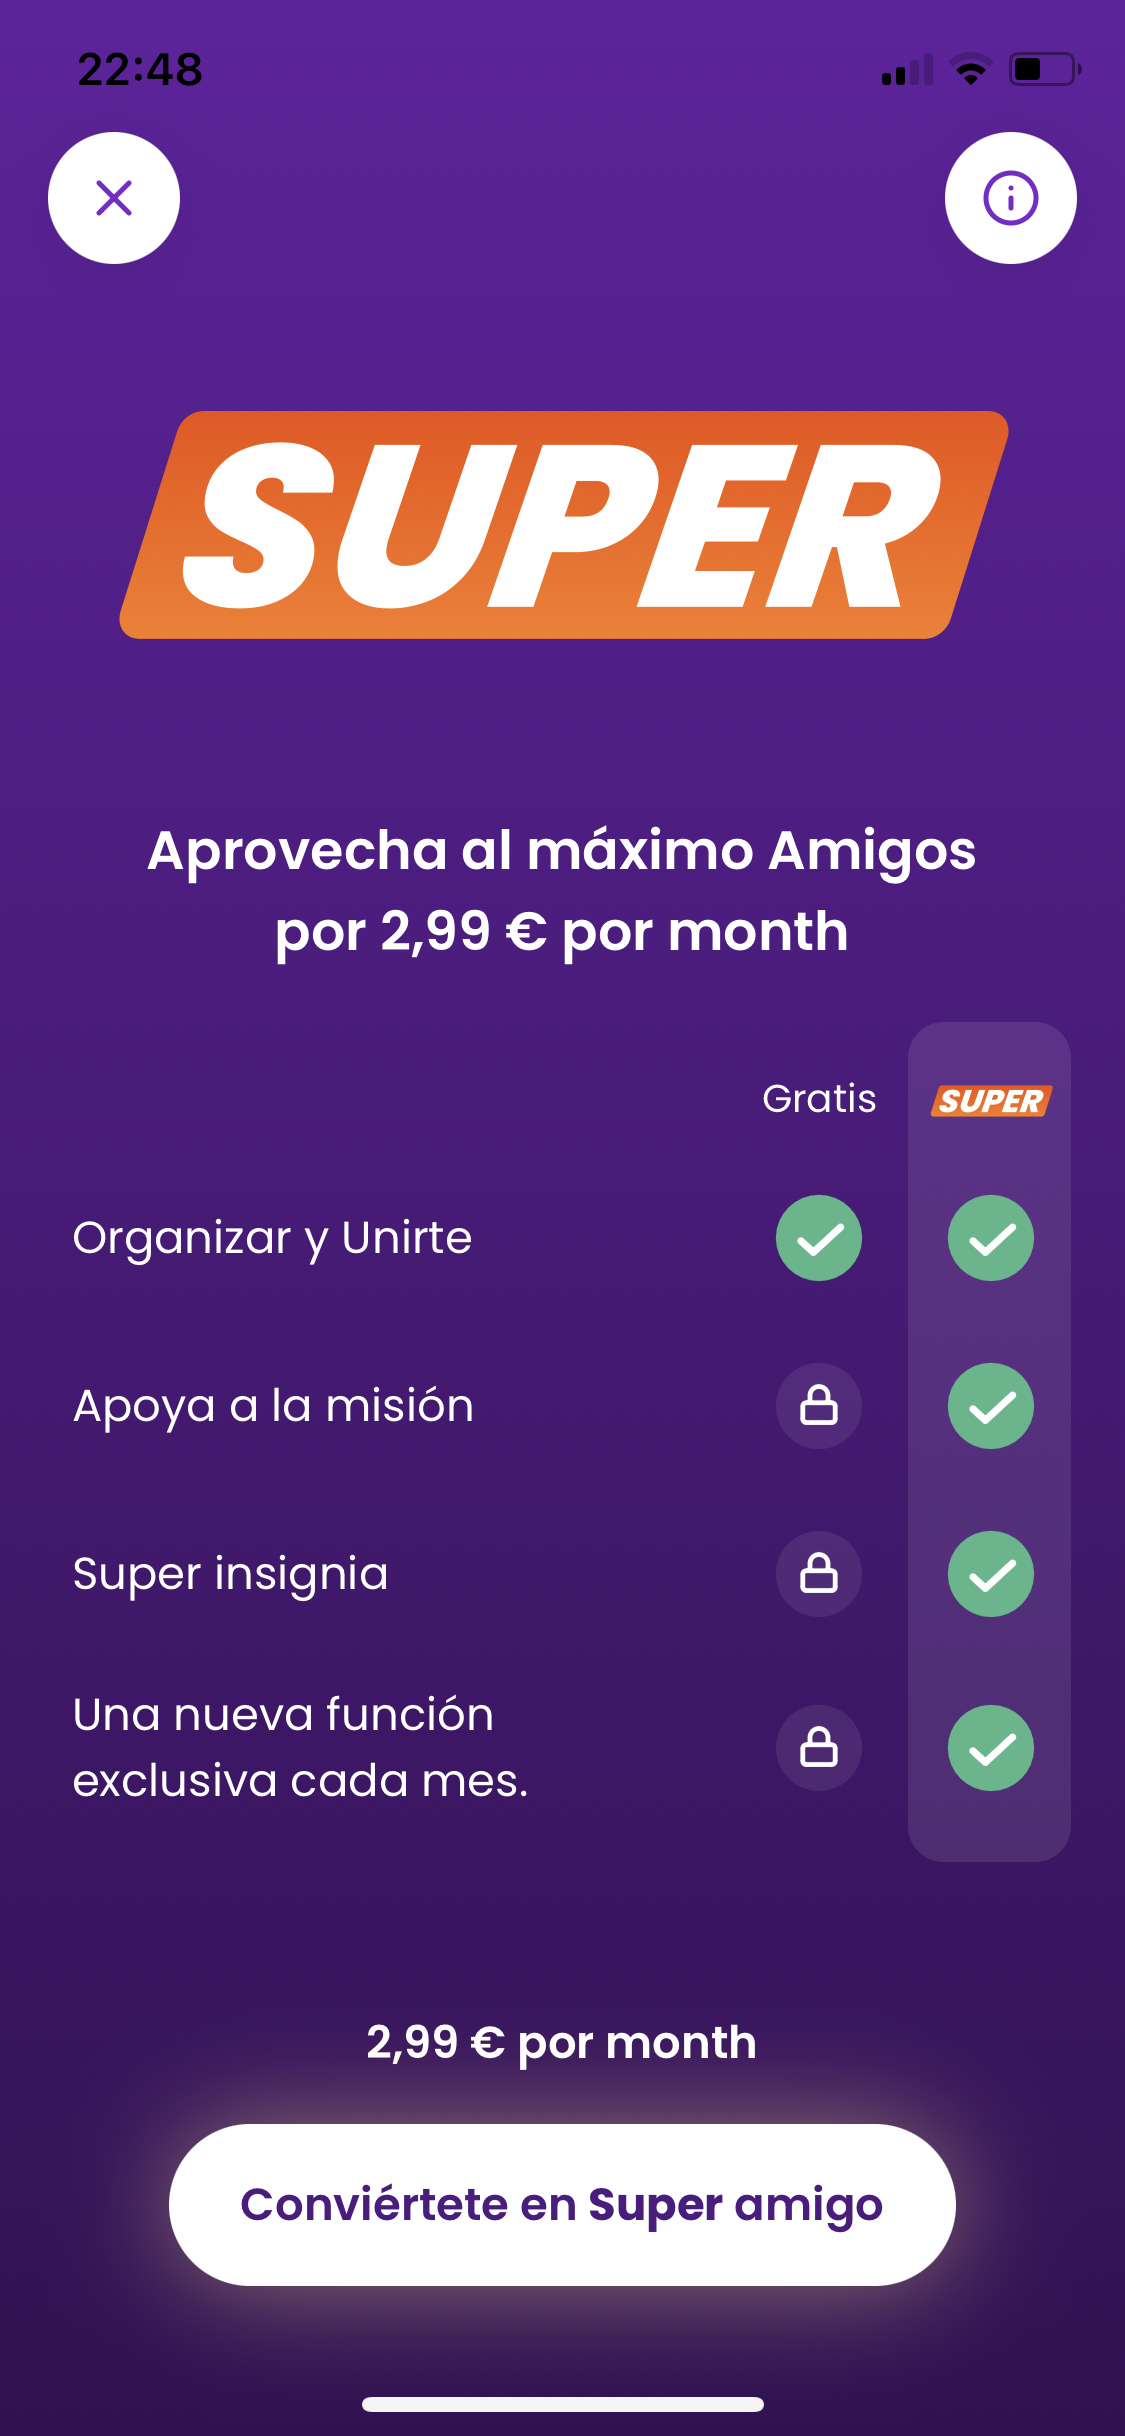
\includegraphics[cframe=black 2pt,width=0.3\linewidth]{images/estadodelarte/amigossocialsuper.jpeg}
  \caption{Amigos Social en la App Store}
  \label{fig:amigosocial_appstore}
\end{figure}

\textbf{Conclusión}

Amigos Social ofrece una alternativa refrescante para aquellos que buscan interacciones sociales genuinas más allá de las limitaciones de los medios sociales tradicionales. Su énfasis en la espontaneidad, eventos locales y una cultura de experiencias compartidas tiene el potencial de fomentar un sentido de comunidad más fuerte dentro de los entornos del mundo real.


\section{Conclusión}

Meetup se centra en fomentar las interacciones en el mundo real a 
través de experiencias compartidas. Sin embargo, su enfoque es más 
general y no está diseñado específicamente para la colaboración en 
proyectos concretos o para la formación de grupos con el objetivo de 
realizar actividades específicas a largo plazo. Además, a pesar de su 
popularidad, Meetup no está exento de críticas, particularmente en lo 
que respecta a la experiencia del usuario y a las tarifas de suscripción 
para los organizadores de grupos.

Strava, por otro lado, es una aplicación que se centra en la
actividad física y la competencia amistosa, proporcionando una
plataforma para que los corredores se conecten, se apoyen
mutuamente y celebren logros. Sin embargo, su enfoque es
más específico y no está diseñado para la colaboración en
proyectos o actividades más allá del ámbito deportivo.

En cambio la propuesta de amigos social resuelve un problema más reciente que padecen las generaciones jóvenes, 
sin embargo, el enfoque de amigos social son interacciones efímeras y más centradas en lo que se podría definir como ocio,
simplemente pasar el rato, charlar, ir de fiesta etc.

Es por ello que notamos que hay una falta de iniciativa que una mezcle aspectos de estas plataformas, es decir que sea enfocado entorno a llevar a cabo proyectos y objetivos específicos, manteniendo la interacción
 social a la vez que fomentando una comunidad con una carácter más emprendedor.

Nuestra propuesta busca abordar estas brechas al proporcionar una 
plataforma más personalizada y simple, orientada a la colaboración en proyectos y 
actividades específicas. A diferencia de Meetup, nuestra aplicación se 
enfoca en la formación de grupos con objetivos a largo plazo y proporcionar
herramientas robustas para la gestión de proyectos y la comunicación en grupo.